\documentclass[a4paper,fleqn]{cas-dc}

\usepackage[authoryear,longnamesfirst]{natbib}
\usepackage{amsmath,amssymb}
\usepackage{xcolor}
\usepackage{placeins}

% ---------------------------------------------------------------------------
% Markers for results that are still being run. Search for \pending and
% \provisional before submission; delete the two lines below to hide them.
\newcommand{\pending}[1]{\textcolor{red}{[PENDING: #1]}}
\newcommand{\provisional}[1]{\textcolor{red}{#1}}
% ---------------------------------------------------------------------------

\ExplSyntaxOn
\cs_set:Npn \__first_footerline:
  { \group_begin: \small \sffamily \__short_authors: :~ { \rmfamily \itshape Honours~Research~Report } \group_end: }
\ExplSyntaxOff
\RenewDocumentCommand\printorcid{}{}

\newcommand{\KL}{D_{\mathrm{KL}}}
\newcommand{\Pa}{\mathrm{Pa}}

\begin{document}
\let\WriteBookmarks\relax

\renewcommand{\textfraction}{.3}
\renewcommand{\topfraction}{.70}
\renewcommand{\bottomfraction}{.50}
\renewcommand{\floatpagefraction}{.60}
\renewcommand{\dbltopfraction}{.60}
\renewcommand{\dblfloatpagefraction}{.60}

\shorttitle{Neural Parameter Estimation for Discrete Bayesian Networks}
\shortauthors{K. Aspoas}

\title [mode = title]{Neural Network Parameter Estimation for Discrete Bayesian Networks with Applications in Medical Diagnosis}



\author[1]{Kaylin Aspoas}
\author[1]{Ritesh Ajoodha\,\textnormal{\itshape (Supervisor)}}
\author[1]{Aashna Gaogle\,\textnormal{\itshape (Co-supervisor)}}

\affiliation[1]{organization={School of Computer Science and Applied Mathematics, University of the Witwatersrand},
            city={Johannesburg},
            country={South Africa}}


\begin{abstract}
Bayesian networks offer an interpretable framework well-suited to medical diagnosis, but their standard parameter estimation methods estimate a separate distribution for every configuration of a variable's parents, and become unreliable when data is scarce relative to the number of configurations. This research replaces the conditional probability table at each node with a neural conditional probability distribution (neural CPD), a small neural network that shares parameters across parent configurations while preserving the interpretable graph structure. Neural CPDs are evaluated against tabular estimators on synthetic networks of varying size, in-degree, sample size and cardinality, and on a real clinical dataset with an expert-elicited structure. On synthetic data, the advantage of neural CPDs grows as the number of training rows per parent configuration falls, and comes from sharing statistical strength rather than storing fewer parameters. On clinical data, neural CPDs outperformed a smoothed tabular estimator at every sample size tested, with the largest gains at finer discretisations.
\end{abstract}

\begin{keywords}
Bayesian networks \sep Parameter estimation \sep Neural networks \sep Medical diagnosis
\end{keywords}

\maketitle

% ===========================================================================
\section{Introduction}\label{sec:intro}
% ===========================================================================

In modern healthcare, medical diagnoses are no longer determined by a doctor alone. Predictive models are increasingly being used to support medical decision making, but this raises a difficult question: Who is to blame when they get it wrong?

In medicine, a diagnosis must be more than an answer: it must be something that can be explained, questioned, and justified. If a model contributes to a missed diagnosis or harmful treatment recommendation, responsibility becomes difficult to assign if there is no reasoning to inspect and no logic to challenge. If predictive models are used to support clinical decisions, they should be held to the same standard we expect of a medical professional.

Unfortunately, many powerful predictive models cannot clearly show their internal reasoning. It is difficult for a clinician to trust a conclusion when they have no way of knowing whether the model has learned a medically meaningful relationship, or whether it has relied on a pattern that is accidental, misleading, or inconsistent with clinical knowledge. Yet predictive models remain invaluable in medical settings. Diagnosis is often shaped by many interacting factors, including symptoms, test results, medical history, medication, and lifestyle, and a well-designed model can help identify patterns that may otherwise be missed. The aim, therefore, is not to replace clinical judgement, but to support it in a way that remains understandable and accountable.

Bayesian networks offer a promising way to approach this problem because they represent medical reasoning as a visible structure of relationships. They can show how different pieces of information are connected and how they contribute to a diagnosis. However, traditional Bayesian networks can struggle when medical relationships become highly complex. Each variable's relationship to its causes is learned as a separate probability for every combination of those causes, and as the number of combinations grows, the data available to estimate each one shrinks. Real diagnosis often depends on many interacting factors, and clinical data rarely grows to match.

This creates the central problem addressed in this research. Deep learning models are powerful enough to capture complex patterns, but they are often difficult to interpret. Bayesian networks are easier to understand, but their traditional learning methods may be too limited for complex medical relationships. To combine these strengths, this research investigates whether neural networks can be used within the interpretable structure of a Bayesian network to improve its ability to capture complex relationships.

The contribution of this work is threefold. First, it characterises where and how tabular estimators such as Maximum Likelihood Estimation (MLE) fail in discrete Bayesian networks, and shows that the failure is governed by the number of training rows available per parent configuration, which falls as in-degree or cardinality increases, or as sample size decreases. Second, it evaluates neural conditional probability distributions (CPDs) as a drop-in replacement for conditional probability tables (CPTs) at cardinalities 2 and 4, reducing divergence from the ground truth by over 8-fold in the most data-scarce regime. Third, it applies the framework to a real clinical dataset with an expert-elicited structure.

The remainder of this report is organised as follows. Section~\ref{sec:related} reviews existing work on interpretable medical prediction, parameter estimation for discrete Bayesian networks, and approaches that combine predictive performance with explainability. Section~\ref{sec:method} presents the methodology, including the experimental design and evaluation approach. Section~\ref{sec:results} presents the results, and Section~\ref{sec:conclusion} concludes and outlines future work.

% ===========================================================================
\section{Related Work}\label{sec:related}
% ===========================================================================

\subsection{Parameter Estimation in Bayesian Networks}

Parameter learning in Bayesian networks with a known DAG reduces to estimating node-wise conditional probability distributions independently. In discrete BNs, MLE estimates each CPT entry as a ratio of observed counts \citep{koller2009probabilistic},
\begin{equation}
\hat{P}(X_i = x_k \mid \Pa(X_i)=u_j)=\frac{N_{ijk}}{N_{ij}},
\label{eq:mle}
\end{equation}
where $N_{ijk}$ counts the samples in which $X_i=x_k$ and $\Pa(X_i)=u_j$. This performs well when data is abundant but fails when parent configurations are unobserved or poorly represented: zero-valued parameters propagate through inference and permanently suppress otherwise valid conclusions \citep{impact_oniko_2013}. The fundamental challenge is the exponential growth of the CPT: a variable with $k$ parents of cardinality $r$ has $r^k$ configurations, and even moderate in-degree produces tables too large to estimate from finite data \citep{learning_oniko_2001,koller2009probabilistic}.

Bayesian parameter estimation with Dirichlet priors ensures non-zero probabilities \citep{koller2009probabilistic}, but specifying informative priors at scale is impractical \citep{comprehensive_kyrimi_2021}. Constraint-based priors such as CaMAP improve on uniform Dirichlet priors but still require expert-provided parameter constraints \citep{constrained_di_2021}. Noisy-OR gates reduce complexity from exponential to linear for binary variables, at the cost of independence assumptions that rarely hold in practice \citep{learning_oniko_2001}. Each of these methods still estimates every parent configuration in isolation or imposes a fixed functional form; none learns how configurations relate to one another from the data.

\subsection{Bayesian Networks in Medical Diagnosis}

BNs are widely applied to medical diagnosis and risk prediction because their graphical structure makes probabilistic reasoning visible and inspectable \citep{comprehensive_kyrimi_2021,zhong2024predicting,bayesian_polotskaya_2024}. In high-stakes clinical environments, model interpretability is a requirement for safe decision making and regulatory compliance \citep{explainable_hulsen_2023}, and post-hoc explanations of black-box models are increasingly criticised as unfaithful to the model's internal reasoning \citep{stop_rudin_2019}. Despite their interpretability, BNs are typically outperformed in predictive accuracy by black-box models, a gap that motivates more expressive parameter estimation methods that preserve the graphical structure.

\subsection{Neural Conditional Modelling}

Neural networks provide a flexible class of function approximators that can parameterise conditional distributions within the factorised structure of a Bayesian network. \citet{Gaogle2026} proposed a Neural-Gaussian Network model in which neural networks replace the conventional linear-Gaussian parameterisation of CPDs in Gaussian BNs, demonstrating that neural parameter estimation is feasible and competitive with classical baselines including ridge regression. However, the Gaussian setting assumes continuous, jointly normal variables, which is rarely satisfied in clinical practice where discrete variables such as symptom presence and categorical risk levels are standard.

This research extends the approach of \citet{Gaogle2026} to the discrete setting, where the exponential scaling of CPTs with parent in-degree and cardinality makes the parameter estimation problem substantially harder. The neural CPD replaces each CPT with a learned function from one-hot-encoded parent variables to a softmax output, sharing parameters across parent configurations while preserving the DAG factorisation.

% ===========================================================================
\section{Methodology}\label{sec:method}
% ===========================================================================

\subsection{Problem Statement}

A Bayesian network is defined by a directed acyclic graph $G$, where each node has an associated conditional probability distribution, and the joint distribution factorises according to $G$ as
\begin{equation}
P(X_1,\dots,X_n)=\prod_{i=1}^{n} P(X_i\mid\Pa_{X_i}),
\end{equation}
where $\Pa_{X_i}$ denotes the parents of $X_i$ in $G$ \citep{koller2007graphical}.

In discrete BNs, methods such as MLE and BPE learn local conditional distributions $P(X_i\mid\Pa_{X_i})$ independently using CPTs. The primary limitation arises from the conditioning on each parent configuration. A variable with $k$ parents of cardinality $r$ has $r^k$ parent configurations, and a separate distribution must be estimated for each. With a fixed amount of data $N$, each configuration is observed on average
\begin{equation}
\rho = \frac{N}{r^{k}},
\label{eq:rho}
\end{equation}
times, so increasing in-degree or cardinality, or reducing the sample size, all reduce $\rho$ in the same way. Once $\rho$ falls near or below one, most configurations are seen rarely or never, and MLE produces zero or uninformed estimates. In medical domains, variables often exhibit complex relationships involving many interacting dependencies, while clinical data does not scale with model complexity. As a result, standard parameter estimation methods are unable to effectively capture the complex, high-dimensional relationships that characterise real-world clinical data.

Although deep learning models are capable of capturing such complex dependencies, their black-box design makes them impractical in clinical settings where medical professionals require transparent reasoning from diagnostic models. The challenge is therefore to develop a parameter learning approach for medical BNs that remains reliable when $\rho$ is small, without sacrificing the interpretability that makes BNs well-suited to clinical decision support.

\subsection{Experimental Design}

The evaluation proceeds in three stages. First, the limitations of tabular estimators are characterised on synthetic networks with controlled in-degree, cardinality, and sample size. Second, neural CPD architectures are compared against MLE on the same synthetic data, and a compact architecture is selected for the main comparison. Third, the framework is applied to a real clinical dataset with an expert-elicited structure, where cardinality is varied through discretisation.

\subsection{Ground-Truth Networks and Synthetic Data}

To evaluate parameter estimation performance under controlled conditions, synthetic datasets are generated from known ground-truth Bayesian networks. This allows the true conditional probability distributions to be known in advance, enabling direct comparison between the learned distributions and the true generating distributions, which would not be possible with real-world medical data.

The ground-truth DAGs are produced by a single generator that controls in-degree directly. The $n$ nodes are shuffled into a random topological order, and the node at position $i$ is given exactly $\min(k,i)$ parents, sampled uniformly from the nodes before it. Every node past the first $k$ therefore has in-degree exactly $k$. Graph density is not targeted, but follows from $n$ and $k$ and is recorded for each realised graph; it ranges from 0.10 ($n=40$, $k=2$) to 1.00 ($n=10$, $k=10$).

Each graph is then parameterised by drawing every column of every ground-truth CPT independently from a symmetric Dirichlet distribution, $P^*(X_i\mid \mathrm{pa}) \sim \mathrm{Dir}(\alpha,\dots,\alpha)$. A smaller $\alpha$ gives sharper, more peaked distributions, and $\alpha = 1$ is uniform over the simplex. Because columns are drawn independently, the ground truth contains no structure shared across parent configurations, which makes it a demanding test for any estimator that relies on sharing.

Table~\ref{tab:grid} lists the experimental settings, which are crossed in full, giving 900 configurations per estimator. To reflect the data scarcity characteristic of real clinical settings, the number of training samples is held constant as in-degree increases, so that any observed degradation in parameter estimation performance is attributable to the growing complexity of the conditional probability space rather than variation in data availability. Five random DAGs are generated per setting.

\begin{table}[tbp]
\caption{Synthetic experimental grid. The binary ($r{=}2$) grid gives 500 configurations for MLE, \texttt{nn\_linear} and \texttt{nn\_32}, and 220 for the tuned networks; the $r{=}4$ subset marked $\dagger$ adds 180 configurations per estimator.}\label{tab:grid}
\begin{tabular*}{\tblwidth}{@{\extracolsep{\fill}}ll@{}}
\toprule
Setting & Values \\
\midrule
Network size $n$ & 10$^\dagger$, 20$^\dagger$, 30$^\dagger$, 40, 50 \\
Parent in-degree $k$ & 2$^\dagger$, 4$^\dagger$, 6$^\dagger$, 8$^\dagger$, 10 \\
Dirichlet $\alpha$ & 0.5$^\dagger$ \\
Training rows $N$ & 200, 600$^\dagger$, 1000$^\dagger$, 1400$^\dagger$ \\
Cardinality $r$ & 2, 4$^\dagger$ \\
DAGs per setting & 5 \\
Test sample (KL only) & 10\,000 rows \\
\bottomrule
\end{tabular*}
\end{table}

Synthetic datasets are generated through ancestral sampling from each ground-truth Bayesian network, and smaller training sets are the first $N$ rows of the largest sample, so they are nested. A separate test sample of 10\,000 rows is drawn from each ground truth and used only to estimate KL divergence; it is never used for fitting or model selection. Every random step (DAG, CPTs, training sample, test sample, train/validation split, and network initialisation) has its own seed derived from the configuration, so results are reproducible and paired across estimators: all estimators see the same networks and data.

\subsection{Parameter Estimation Methods}

\subsubsection{Tabular Estimators}

The primary baseline is Maximum Likelihood Estimation, which estimates CPT parameters with Eq.~\eqref{eq:mle} over the full state space. A parent configuration that never appears in the data is assigned a uniform distribution. A child state never observed under an observed configuration keeps a probability of zero, which is floored at $10^{-12}$ when divergences are computed.

Bayesian parameter estimation (BPE) avoids these zeros by adding a symmetric Dirichlet pseudocount of 0.5 to every cell before normalising, $\hat P = (N_{ijk}+0.5)/(N_{ij}+0.5r)$. This Dirichlet estimator is included alongside MLE in the synthetic failure analysis, and is the main tabular baseline on real data, where plain MLE's zero probabilities dominate the score.

\subsubsection{Neural CPDs}

To address the limitations of tabular CPT parameterisation, the local conditional probability table is replaced with a neural-network-based CPD. For each node $X_i$, a neural network $f_\theta$ is trained to approximate $P(X_i\mid\Pa(X_i))$, where the parent variables are provided as input features. The neural CPD therefore learns a functional mapping
\begin{equation}
P(X_i\mid\Pa(X_i))=f_\theta(\Pa(X_i)),
\end{equation}
parameterised by neural network weights $\theta$. Each parent is one-hot encoded at its own cardinality and the encodings are concatenated, so the input width grows with the \emph{sum} of parent cardinalities rather than their product. A root node receives a constant zero input and learns its marginal through the output bias. Hidden layers compute $h=\phi(Wx+b)$ with ReLU activation $\phi$, and the output layer uses a softmax activation function to produce a valid probability distribution over the discrete states of $X_i$ \citep{goodfellow2016deep},
\begin{equation}
\hat{y}=\mathrm{softmax}(W_{\mathrm{out}}h+b_{\mathrm{out}}).
\end{equation}
This allows the neural network to approximate discrete conditional probability distributions while sharing parameters across parent configurations. The neural CPDs are trained using cross-entropy loss,
\begin{equation}
\mathcal{L}(\theta)=-\frac{1}{N}\sum_{s=1}^{N}\log P_\theta\big(x_i^{(s)} \mid \mathrm{pa}_i^{(s)}\big),
\end{equation}
where $x_i^{(s)}$ is the observed node state and $\mathrm{pa}_i^{(s)}$ is the observed parent configuration \citep{goodfellow2016deep}. One network is trained per node. For neural CPDs, 20\% of the training rows are held out as a validation subset, and each node is early-stopped independently on validation cross-entropy. MLE fits on all $N$ rows, so the neural estimators see fewer rows, not more.

Table~\ref{tab:estimators} lists the estimators. The linear softmax, with no hidden layer, is equivalent to L2-penalised multinomial logistic regression fitted per node; it shares parameters across configurations but cannot represent interactions between parents, and so acts as a control for the effect of the hidden layer. \texttt{nn\_32} has a single hidden layer of 32 units with default settings, and the two deeper networks were selected by the tuning procedure below.

\begin{table}[tbp]
\caption{Estimators. Untuned networks use Adam \citep{kingma2015adam} with weight decay $10^{-4}$, batch size 64 and patience 20; tuned networks use AdamW \citep{loshchilov2019decoupled} with weight decay 0.01.}\label{tab:estimators}
\begin{tabular*}{\tblwidth}{@{\extracolsep{\fill}}llp{3.1cm}@{}}
\toprule
Estimator & Form & Settings \\
\midrule
\texttt{mle} & CPT & Uniform for unseen configurations \\
\texttt{dirichlet} & CPT & Pseudocount 0.5 \\
\texttt{nn\_linear} & No hidden layer & Tuned per cardinality \\
\texttt{nn\_32} & 32 ReLU & Tuned per cardinality \\
\texttt{nn\_64\_32} & 64--32 ReLU & Tuned per cardinality \\
\texttt{nn\_128\_64} & 128--64 ReLU & Tuned per cardinality \\
\texttt{nn\_256} & 256 ReLU & Tuned per cardinality \\
\bottomrule
\end{tabular*}
\end{table}

\subsection{Neural CPD Architecture Selection}

Architecture selection proceeded in three stages. First, an initial sweep of fixed architectures was run without early stopping at $k=10$ to establish overfitting behaviour (Supplementary Figure~S1). Larger networks overfit quickly, confirming that early stopping on validation loss is essential; every network in the main experiments uses it.

Second, Bayesian hyperparameter sweeps were conducted separately for $r=2$ and $r=4$, each at multiple in-degrees (Supplementary Figure~S2). For $r=2$, sweeps at $k=6$ and $k=10$ covered learning rate, hidden layers, dropout, weight decay, batch size and patience, each trial scored by mean KL over five tuning DAGs. For $r=4$, analogous sweeps were run at $k=2$, $k=6$ and $k=10$. At both cardinalities, moderately large single-layer networks (256 units) and two-layer networks (128--64, 256--128) dominated the sweeps, with learning rates near $3$--$6\times10^{-4}$.

Third, the best sweep configurations were re-run on every tuning setting to select final candidates. The tuned configurations were retained for the architecture comparison, but the main synthetic comparison uses \texttt{nn\_32}, a single hidden layer of 32~units. Although \texttt{nn\_32} is not the most accurate architecture, it performs within 30\% of the best tuned network at $r=4$ and the gap narrows as the number of parent configurations grows, while holding up to 66 times fewer parameters and training substantially faster. All tuning was performed on a separate set of tuning DAGs disjoint from the evaluation DAGs, so no evaluation test set influenced any choice.

\subsection{Real-World Application}

The real-data component uses the CDC Diabetes Health Indicators dataset \citep{cdc_diabetes_2023}, drawn from the 2015 Behavioral Risk Factor Surveillance System (BRFSS), comprising 253\,680 survey responses across 21 health-related variables and a binary diabetes indicator. BRFSS is publicly available, fully de-identified, and exempt from institutional review board oversight.

The graph structure for this dataset is taken from the expert-elicited diabetes DAGs published by \citet{zahoor2024investigatingvaliditystructurelearning}, at three expert-confidence levels (Supplementary Figure~S3). Only the DAG is taken from experts; all parameters are learned.

Because responses are collected by a structured survey instrument, every variable except body mass index is natively categorical, so the discretisations compared are defined by the survey instrument rather than chosen here. The coarsest setting (L1) reproduces the collapsing applied in practice to keep conditional probability tables estimable, and matches the published marginals to within one percentage point. L2 uses the categories as collected (for example, 13 age bands, 8 income bands and the WHO body mass index classes), and L3 additionally bins body mass index and the day-count variables more finely. Varying discretisation therefore varies $\rho$ through cardinality, with the graph held fixed.

On this data, estimator performance is assessed by three-fold cross-validation, stratified on diabetes status. Within each training fold, nested subsets of $N\in\{500, 2000, 10\,000, 50\,000\}$ rows are drawn, allowing the ratio of parent configurations to available samples to be varied independently of discretisation granularity. Neural CPDs hold out 20\% of each subset for early stopping, so no test fold influences model selection. All nine combinations of discretisation (L1, L2, L3) and DAG confidence (high, moderate, low) are evaluated.

\subsection{Evaluation}

The primary metric for the synthetic experiments is the Kullback-Leibler divergence between the ground-truth joint distribution $P^*$ and the learned distribution $\hat P$ \citep{koller2009probabilistic}. The sum over all $r^n$ joint states is intractable at these network sizes, so the chain-rule decomposition is used, with a Monte Carlo estimate over the $S=10\,000$ test rows $x^{(s)}\sim P^*$:
\begin{align}
\KL(P^*\|\hat P) &= \mathbb{E}_{P^*}\Big[\sum_{i} \KL\big(P^*_{i}\,\|\,\hat P_{i}\big)\Big] \nonumber\\
&\approx \frac{1}{S}\sum_{s=1}^{S}\sum_{i=1}^{n}\sum_{x_i} P^*_{is}(x_i)\log\frac{P^*_{is}(x_i)}{\hat P_{is}(x_i)},
\end{align}
where $P^*_{i}$ and $\hat P_{i}$ are the true and learned distributions of $X_i$ given its parents, and $P^*_{is}(x_i) = P^*(x_i\mid \mathrm{pa}_i^{(s)})$, with $\hat P_{is}$ defined likewise.
The inner sum over each child's states is exact; only the parent configurations are sampled. Because KL is summed over nodes it scales with network size, so it is reported per node where network sizes are compared.

Since the ground-truth conditional distributions are unavailable for real data, predictive performance is assessed by the mean held-out log-likelihood per row, $\frac{1}{S}\sum_s\sum_i \log\hat P(x_i^{(s)}\mid\mathrm{pa}_i^{(s)})$. The expected held-out negative log-likelihood is the cross-entropy $H(P^*,\hat P) = H(P^*) + \KL(P^*\,\|\,\hat P)$, and since $H(P^*)$ does not depend on the estimator, differences in log-likelihood are exactly differences in KL divergence. The ranking of estimators therefore transfers from the synthetic setting, while the absolute divergence from truth does not. The unseen-configuration rate, the fraction of test parent configurations never observed in training, is also reported.

Alongside these measures of accuracy, the computational cost of each estimator is recorded. Free parameters are counted as $(r-1)$ times the number of configurations for a CPT, and every weight and bias for a network. Training time is recorded separately in a serial run, since parallel execution inflates wall-clock times.

\section{Results}\label{sec:results}

\subsection{How Tabular Methods Fail}

The synthetic setup reproduces the well-known behaviour of tabular estimators under sparse data \citep{learning_oniko_2001,koller2009probabilistic}. Both MLE and the Dirichlet estimator estimate each parent configuration from its own counts, so their CPTs grow exponentially with in-degree. Figure~\ref{fig:mle} shows that, for MLE, KL divergence and CPT memory both rise sharply once a node's parent configurations ($2^k$) outnumber the training rows: in 40-node networks, KL rises from 0.28 to 58 nats and memory from 2.5 to 508\,KB as in-degree goes from 2 to 10. \pending{Dirichlet KL divergence as in-degree increases.}

\begin{figure}[pos=tbp]
\centering
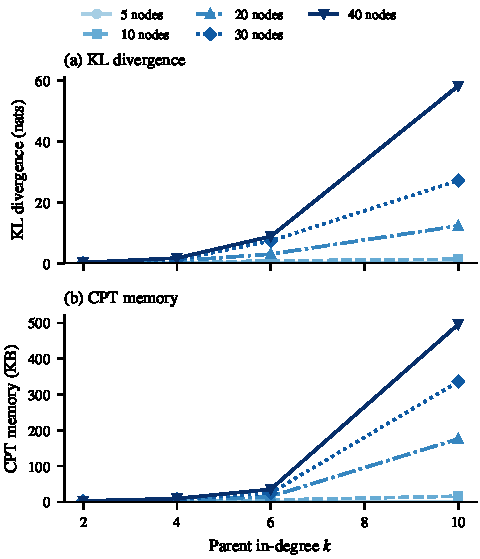
\includegraphics[width=\columnwidth]{figs/mle_fails.pdf}
\caption{MLE on synthetic networks ($r=2$) as in-degree increases ($N=1000$, $\alpha=0.5$, mean over five DAGs; darker is larger). (a) KL divergence to the ground truth. (b) Total CPT memory.}\label{fig:mle}
\end{figure}

The cause is data coverage rather than computation. In 20-node networks at $N=1000$, the share of parent configurations never seen in training rises from 0.5\% at $k=2$ to 78\% at $k=10$, while every MLE fit takes under one second. Both tabular estimators assign a uniform distribution to every unseen configuration, since the Dirichlet pseudocount alone carries no information about it, so smoothing removes zero probabilities but cannot recover these columns. Tabular estimation therefore degrades smoothly as the number of rows per parent configuration falls.

\FloatBarrier
\subsection{Neural CPD Architectures}

Figure~\ref{fig:arms} compares every neural architecture with MLE on the configurations shared by all estimators at both $r=2$ and $r=4$, using the number of parent configurations $r^k$ as the x-axis to unify the effect of in-degree and cardinality. All MLPs achieve lower KL divergence than MLE across the full range of $r^k$, and the gap widens as the configuration space grows.

\begin{figure*}[pos=tbp]
\centering
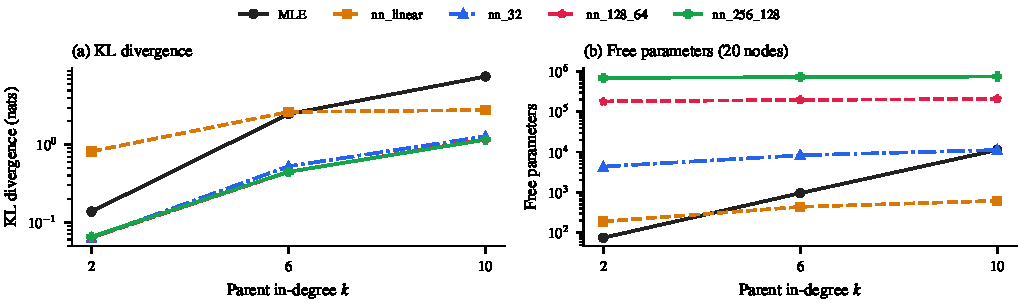
\includegraphics[width=\textwidth]{figs/arms.pdf}
\caption{All estimators on the shared configurations at $r\in\{2,4\}$ (10--30 nodes, $\alpha=0.5$, $N\in\{600,1000,1400\}$; log-scaled axes). (a) Mean KL divergence vs.\ the number of parent configurations $r^k$. (b) Free parameters for a 20-node network.}\label{fig:arms}
\end{figure*}

The linear softmax is the useful control: it shares parameters across parent configurations but has no hidden layer, and so cannot represent interactions between parents. It is worse than MLE at small $r^k$ and only overtakes it when the configuration space is large enough. Parameter sharing alone is therefore not the mechanism; the hidden layer is.

Figure~\ref{fig:arms}(b) shows the cost of each estimator in free parameters. The CPT grows exponentially with $r^k$, while the networks grow only linearly, because their input width is the sum rather than the product of parent cardinalities. Even so, the tuned networks hold far more parameters than the tables they replace: \texttt{nn\_256} holds 89\,896 free parameters at $k=10$, $r=2$, eight times as many as the CPT's 11\,263. Neural CPDs therefore do not save parameters. What they save is data, by sharing statistical strength across parent configurations, which is a statistical-efficiency argument rather than a storage one.

The differences between the MLPs are small by comparison. At $r=2$, \texttt{nn\_32} averages 1.95 times the KL of the best tuned architecture across settings, but at $r=4$ the gap narrows: \texttt{nn\_32} is within 3\% of the best at high in-degree ($k\geq6$) and within 30\% even at $k=2$. The architecture choice is also stable across cardinalities: \texttt{nn\_256} and \texttt{nn\_128\_64} alternate as the best tuned network at both $r=2$ and $r=4$, and the ranking among the MLPs does not change with sample size or in-degree. Because \texttt{nn\_32} holds up to 66 times fewer parameters, trains substantially faster (mean 202\,s vs.\ $>$900\,s per network), and is the most robust to overfitting (Supplementary Figure~S1), it is used as the neural CPD for the remainder of the synthetic results.

\FloatBarrier
\subsection{Neural CPDs Compared with MLE}

Figure~\ref{fig:klN} shows how each estimator responds to more data. More rows help MLE, but at high in-degree it stays far worse than \texttt{nn\_32}. At $k=2$ MLE and \texttt{nn\_32} improve at a similar rate, and the gap stays roughly constant. Across the $r=2$ grid, \texttt{nn\_32} beats MLE in 98.8\% of 500 configurations, rising from 94\% at $k=2$ to 100\% at $k\geq4$.

\begin{figure*}[pos=tbp]
\centering
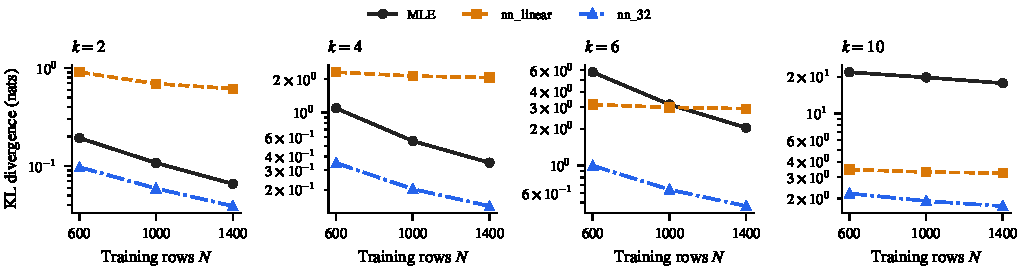
\includegraphics[width=\textwidth]{figs/kl_vs_N.pdf}
\caption{KL divergence against training rows at each in-degree ($r=2$, mean over all network sizes and five DAGs; log-scaled y-axis).}\label{fig:klN}
\end{figure*}

Figure~\ref{fig:sizealpha} shows KL divergence over different ground-truth distributions. MLE degrades fastest with network size and with flatter true CPTs. As networks grow from 5 to 40 nodes, MLE's mean KL rises from 0.05 to 15.7 nats against 0.02 to 1.85 for \texttt{nn\_32}, so the ratio between them grows from 2.8 to 8.5. Peaked ground truths ($\alpha=0.1$) concentrate the data on fewer configurations and keep MLE's error low, at 1.9 times that of \texttt{nn\_32}. Flat ground truths ($\alpha=1$) spread the data across all configurations, and MLE's error rises to 12 times that of \texttt{nn\_32}, which is largely insensitive to $\alpha$.

\begin{figure*}[pos=tbp]
\centering
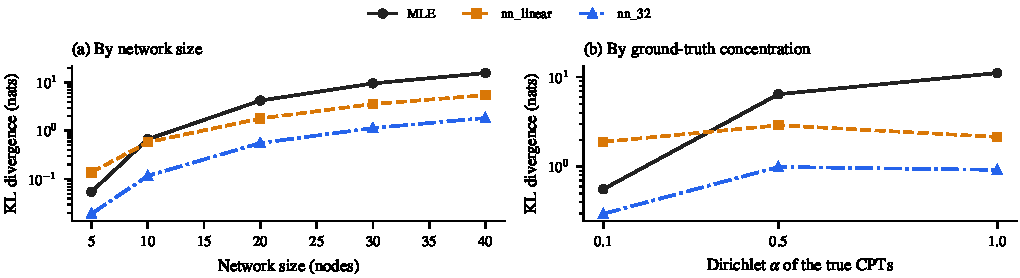
\includegraphics[width=\textwidth]{figs/size_alpha.pdf}
\caption{Mean KL divergence (log-scaled y-axis), (a) by parent in-degree ($r=2$, all network sizes and sample sizes) and (b) by the Dirichlet concentration $\alpha$ of the true CPTs ($r=2$).}\label{fig:sizealpha}
\end{figure*}

In-degree, cardinality and sample size all act on the estimators through the number of rows per parent configuration, $\rho=N/r^k$ (Eq.~\ref{eq:rho}). Figure~\ref{fig:rho} plots the ratio of MLE's KL to \texttt{nn\_32}'s against $\rho$ for every $(k,N)$ setting at $r=2$, pooling across network sizes and DAGs. The advantage of the neural CPD falls steadily as $\rho$ increases, from over 6 times at $\rho\approx0.2$ to roughly 2 times at $\rho=350$, and the settings from different in-degrees join into a single decreasing trend. The neural CPD is most valuable exactly where data per configuration is scarcest.

The $r=4$ experiments confirm that the same pattern holds at higher cardinality: \texttt{nn\_32} beats MLE in all 180 configurations tested, and the architecture ranking is also stable, with \texttt{nn\_32} within 3\% of the best tuned network at $k\geq6$.

\begin{figure}[pos=tbp]
\centering
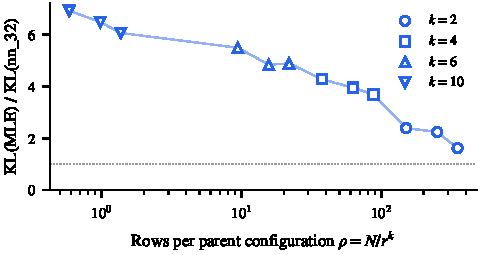
\includegraphics[width=\columnwidth]{figs/rho.pdf}
\caption{Ratio of MLE to \texttt{nn\_32} KL divergence against rows per parent configuration $\rho = N/2^k$ ($r=2$, mean over all network sizes and DAGs; log-scaled x-axis).}\label{fig:rho}
\end{figure}

The same advantage can be expressed as data efficiency. Table~\ref{tab:isokl} shows the training rows needed for each estimator to reach a KL divergence of 5.0~nats, interpolated from the mean KL at each sample size ($r=2$). At $k=4$, MLE needs 458 rows against fewer than 200 for \texttt{nn\_32}. At $k\geq8$, MLE and the linear softmax cannot reach this threshold at any sample size in the grid, whereas \texttt{nn\_32} reaches it at 462 rows ($k=8$) and 918 rows ($k=10$).

This data efficiency comes at a computational cost, since neural CPDs are more expensive to train. MLE fits in under one second at every setting; \texttt{nn\_32} averages 202\,s per network (up to 930\,s at the largest settings), and the tuned networks take longer still. The cost is per-node and dominated by early-stopping patience at high in-degree, where fewer epochs are needed before validation loss plateaus.

\begin{table}[tbp]
\caption{Training rows $N$ needed to reach KL $\leq 5.0$ nats ($r=2$, interpolated from mean KL at each sample size). Entries marked $>$1400 indicate that the threshold was not reached within the grid.}\label{tab:isokl}
\begin{tabular*}{\tblwidth}{@{\extracolsep{\fill}}rrrr@{}}
\toprule
$k$ & MLE & \texttt{nn\_linear} & \texttt{nn\_32} \\
\midrule
2 & $<$200 & $<$200 & $<$200 \\
4 & 458 & 320 & $<$200 \\
6 & 1275 & $>$1400 & $<$200 \\
8 & $>$1400 & $>$1400 & 462 \\
10 & $>$1400 & $>$1400 & 918 \\
\bottomrule
\end{tabular*}
\end{table}

\FloatBarrier
\subsection{Real Clinical Data}

\subsubsection{Size of the Estimation Problem}

Supplementary Figure~S3 shows the expert-elicited structure. The high-confidence graph has 37 edges and a maximum in-degree of 7, with Smoker, Fruits and Veggies unconnected; the moderate-confidence graph adds 13 edges, for a maximum in-degree of 8 at the diabetes node; and the low-confidence graph has 55 edges and a maximum in-degree of 12.

Table~\ref{tab:realconfig} shows how discretisation and graph confidence change the size of the estimation problem. Refining the discretisation from L1 to L2 multiplies the number of free CPT parameters by 5.4 on the high-confidence graph and by 10.6 on the moderate-confidence graph, while the neural input width grows by less than two-fold.

\begin{table*}[tbp]
\caption{Size of the real-data estimation problem for each discretisation and expert DAG.}\label{tab:realconfig}
\begin{tabular*}{\tblwidth}{@{\extracolsep{\fill}}llrrrr@{}}
\toprule
Discretisation & DAG & Max in-degree & Edges & CPT parameters & NN input width \\
\midrule
L1 & High & 7 & 37 & 1\,348 & 129 \\
L1 & Moderate & 8 & 50 & 4\,654 & 162 \\
L1 & Low & 12 & 55 & 95\,392 & 176 \\
L2 & High & 7 & 37 & 7\,310 & 214 \\
L2 & Moderate & 8 & 50 & 49\,496 & 261 \\
L2 & Low & 12 & 55 & 1\,622\,067 & 281 \\
L3 & High & 7 & 37 & 15\,576 & 232 \\
L3 & Moderate & 8 & 50 & 93\,550 & 285 \\
L3 & Low & 12 & 55 & 9\,016\,841 & 309 \\
\bottomrule
\end{tabular*}
\end{table*}

\subsubsection{Predictive Performance}

The real-data experiments used MLE, a Dirichlet estimator (pseudocount 0.5), the linear softmax, \texttt{nn\_32}, and \texttt{nn\_128\_64}, evaluated by three-fold cross-validation across all nine combinations of discretisation (L1, L2, L3) and DAG confidence (high, moderate, low).

Figure~\ref{fig:realmean} shows held-out log-likelihood averaged over all settings. Plain MLE is far below every other estimator at small $N$, because unseen child states receive near-zero probability. All three neural architectures outperform the Dirichlet estimator at every sample size, and perform nearly identically to one another.

\begin{figure}[pos=tbp]
\centering
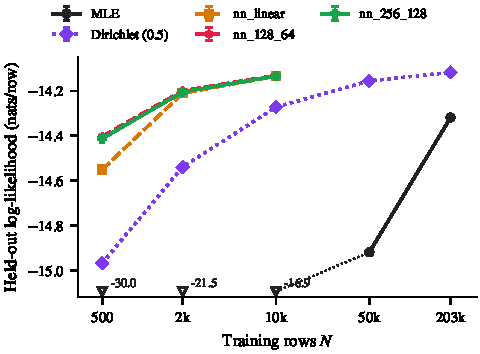
\includegraphics[width=\columnwidth]{figs/real_mean.pdf}
\caption{Held-out log-likelihood per row, mean over all nine settings and three folds (higher is better; log-scaled x-axis).}\label{fig:realmean}
\end{figure}

Figure~\ref{fig:real} breaks this down across all nine discretisation and DAG combinations. MLE is excluded to keep the y-axis range informative. The rows correspond to discretisation levels (L1, L2, L3) and columns to DAG confidence (high, moderate, low). Moving down (finer discretisation) or right (denser graph) increases the number of parent configurations and widens the gap between the neural estimators and the Dirichlet baseline. At the extremes (L3 with the low-confidence graph), the Dirichlet estimator's log-likelihood is 0.6~nats per row worse than the neural estimators at $N=500$.

\begin{figure*}[pos=tbp]
\centering
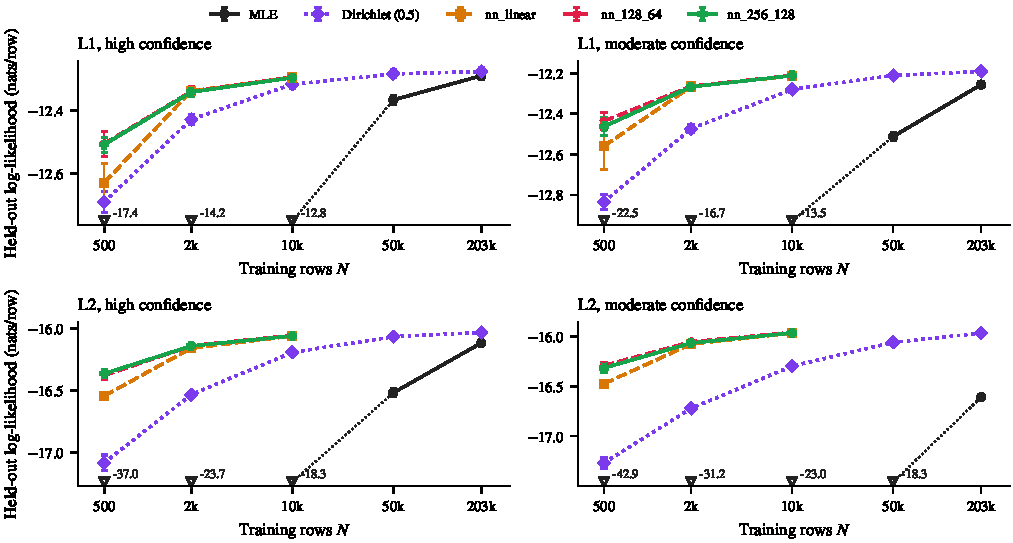
\includegraphics[width=\textwidth]{figs/real_loglik.pdf}
\caption{Held-out log-likelihood per row for each discretisation (rows) and DAG confidence (columns), excluding MLE (mean $\pm$ s.d.\ over three folds; log-scaled x-axis).}\label{fig:real}
\end{figure*}

Unlike the synthetic experiments, the linear softmax is competitive with \texttt{nn\_32} and \texttt{nn\_128\_64} on real data. Survey variables such as age, income and body mass index are ordinal and act on outcomes in largely monotone ways that an additive model can capture, whereas the synthetic ground-truth CPT columns were drawn independently.

The gap between the tabular and neural estimators follows from data coverage. Supplementary Figure~S4 shows the fraction of test parent configurations unseen in training; it rises sharply with finer discretisation and denser graphs, explaining why MLE and the Dirichlet estimator fall behind at small $N$.

\subsubsection{Parameter and Training Cost}

Figure~\ref{fig:realparams} shows the parameter cost of each estimator across the nine settings, analogous to Figure~\ref{fig:arms}(b) for the synthetic data. The CPT grows by orders of magnitude as discretisation becomes finer and the graph becomes denser, from 1\,348 parameters (L1, high) to over 9 million (L3, low), whereas the neural networks grow slowly because their input width scales with the sum rather than the product of parent cardinalities. At the densest setting, \texttt{nn\_32} holds 13\,364 parameters against the CPT's 9\,016\,841.

\begin{figure}[pos=tbp]
\centering
\includegraphics[width=\columnwidth]{figs/real_params.pdf}
\caption{Free parameters for each estimator on the real data, plotted against the CPT size (tabular complexity) for the same discretisation and DAG (log-scaled axes). The diagonal line marks equal parameter count.}\label{fig:realparams}
\end{figure}

The smaller parameter count does not make the neural estimators cheaper to fit. Figure~\ref{fig:timing} shows fit time on the real data. MLE and the Dirichlet estimator fit in under a minute at every sample size. The neural estimators scale with $N$: \texttt{nn\_32} takes 14\,s at $N=500$ and 122\,s at $N=50\,000$, while \texttt{nn\_128\_64} reaches 270\,s at $N=50\,000$. The cost is acceptable for a one-off fit but would need consideration in an iterative or online setting.

\begin{figure}[pos=tbp]
\centering
\includegraphics[width=\columnwidth]{figs/real_timing.pdf}
\caption{Fit time on the real dataset (mean $\pm$ s.d.\ over three folds across all discretisation and DAG settings; log-scaled axes).}\label{fig:timing}
\end{figure}

% ===========================================================================
\FloatBarrier
\section{Conclusion and Future Work}\label{sec:conclusion}
% ===========================================================================

Medical diagnosis is a high-stakes domain where predictive models must be not only accurate but transparent. Bayesian networks are among the most promising frameworks for this setting, because their graphical structure makes probabilistic reasoning visible and inspectable. Yet this promise is undermined by a fundamental limitation: standard parameter estimation methods estimate every parent configuration from its own observations, and cannot reliably capture high-dimensional dependencies when data is scarce relative to the number of configurations.

This report addressed that limitation by replacing traditional conditional probability tables with neural-network-based conditional probability distributions, retaining the interpretable graphical structure of Bayesian networks while leveraging the representational power of deep learning for local parameter estimation. Neural CPDs reduced KL divergence from the ground truth across both cardinalities tested ($r=2$ and $r=4$), and their advantage over tabular estimation grew as the number of rows per parent configuration fell, with the $r=4$ results following the same trend as $r=2$. On real clinical data, neural CPDs outperformed smoothed tabular estimation at every sample size tested, with the largest gains at the finer discretisation, which suggests that collapsing clinical categories to keep CPTs estimable is less necessary when local distributions are learned by neural networks. Across all experiments, a single quantity, the number of rows per parent configuration, unifies the effects of in-degree, cardinality and sample size. The benefit of neural CPDs is statistical efficiency rather than compactness: the networks hold more parameters than the tables they replace, but need far less data to estimate them well.

\subsection{Limitations}

The synthetic networks use cardinalities of 2 and 4 with a fixed in-degree per node and independently drawn Dirichlet CPTs; they do not reproduce the noise, correlation structure or class imbalance of clinical data, which the real-data experiment addresses only in part. \provisional{A smoothed tabular estimator was not included in the synthetic grid,} the tuned networks were run on a subset of it, and hyperparameters were tuned separately for each cardinality at $n=20$ and $\alpha=0.5$. Continuous variables must be discretised, which loses information. Finally, a neural CPD is less directly readable than a CPT: the graph remains interpretable, but each local distribution has to be queried rather than read off a table.

\subsection{Future Work}

The most natural extension is to continuous and hybrid networks. Many physiological measurements, such as blood pressure, glucose and body mass index, are continuous, and discretising them loses information. \citet{Gaogle2026} showed that neural CPDs are effective for Gaussian Bayesian networks, and this report shows the same for discrete networks; combining the two into hybrid networks with neural CPDs for both continuous and discrete children would let clinical variables be modelled in their natural form, with the graph remaining the interpretable part of the model.

A second direction is richer clinical data. Critical care databases such as MIMIC contain far more variables and rarer conditions than BRFSS, which is exactly the regime of few rows per parent configuration in which neural CPDs were most valuable here, and where class imbalance makes zero-probability estimates most harmful.

Neural CPDs could also be combined with expert knowledge. Monotonicity or sign constraints on the networks, elicited from clinicians, would encode accepted medical relationships directly, and the same networks could be learned jointly with the graph during structure learning rather than fitted to a fixed structure.

Finally, the value of a diagnostic model lies in the queries it answers. Evaluating posterior diagnostic probabilities computed through the fitted networks, and presenting a neural CPD to clinicians as a table generated on demand for the configurations they ask about, would test whether the gains in local estimation carry through to clinical decision support.

\clearpage
\bibliographystyle{cas-model2-names}
\bibliography{references}

\end{document}
